\originalsection{扩展数据}\label{alphaproof-extended-data}
\begin{center}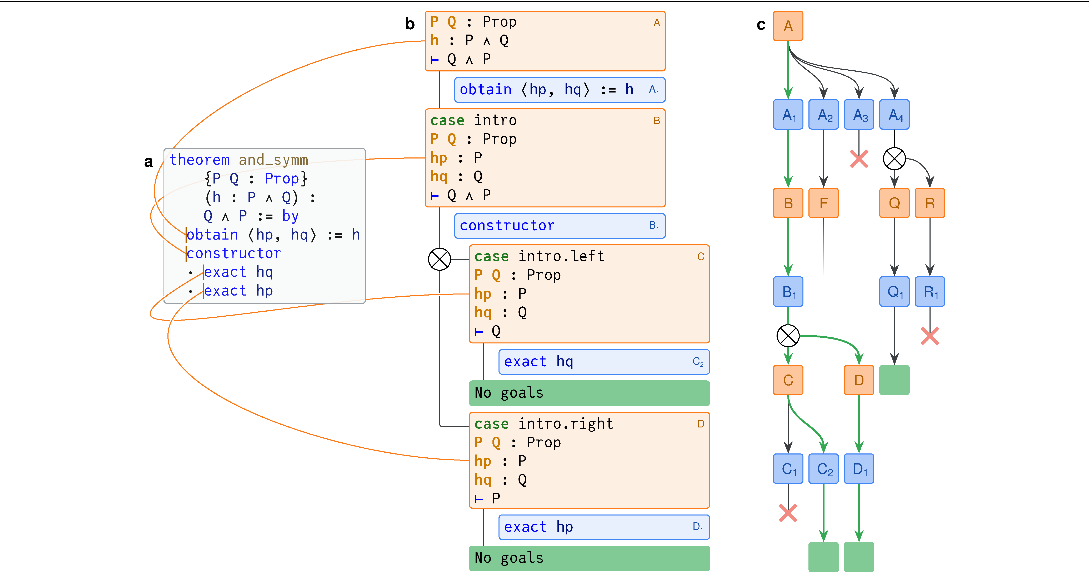
\includegraphics[width=\linewidth]{../papers/translations/alphaproof/assets/edfig1.pdf}\end{center}
\phantomsection
\noindent\textbf{扩展数据图 1. Lean tactic 环境及其树搜索建模.}\paperlabel{扩展数据 1}{alphaproof-edfig1}
a, Lean 编辑器环境, 光标位置关联 tactic 状态信息. b, 对应证明树, 通过动作 (tactic) 连接观测 (tactic 状态). $\otimes$ 表示有多个必须全部解决的子目标. c, 搜索树, 粗绿箭头高亮找到的成功证明.

\noindent\textbf{图中文字对应.} No goals: 无剩余目标. a 面板完整代码保持原样: 对命题 $P,Q$ 证明 $Q\land P$; 先从假设 $P\land Q$ 取出 \texttt{hp,hq}, 用 \texttt{constructor} 分开合取目标, 分别由 \texttt{exact hq}、\texttt{exact hp} 完成. b 的所有假设、目标、\texttt{case intro}、\texttt{case intro.left}、\texttt{case intro.right} 状态与 A--D 编号, c 的全部节点、失败叉号和 AND 符号均以原图保留.

\begin{center}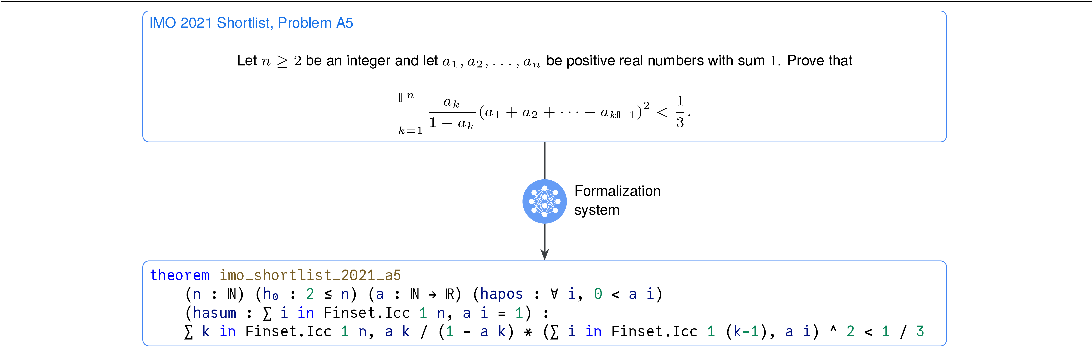
\includegraphics[width=\linewidth]{../papers/translations/alphaproof/assets/edfig2.pdf}\end{center}
\phantomsection
\noindent\textbf{扩展数据图 2. 自动形式化过程的一个例子.}\paperlabel{扩展数据 2}{alphaproof-edfig2}
原文图 2a 的形式化系统接收以 LaTeX 排版的自然语言题面, 输出有效 Lean 代码形式命题. 署名: Google DeepMind.

\noindent\textbf{图内题面完整中译.} IMO 2021 候选题, A5. 设整数 $n\ge2$, 正实数 $a_1,\ldots,a_n$ 的和为 1. 证明
\[
\sum_{k=1}^n\frac{a_k}{1-a_k}(a_1+a_2+\cdots+a_{k-1})^2<\frac13.
\]
Formalization system: 形式化系统. 下方完整 Lean 命题, 包括 $n$ 类型、$h_0$、$a$、\texttt{hapos}、\texttt{hasum}、有限集合求和上下界及目标不等式, 按原图保留.

\begin{center}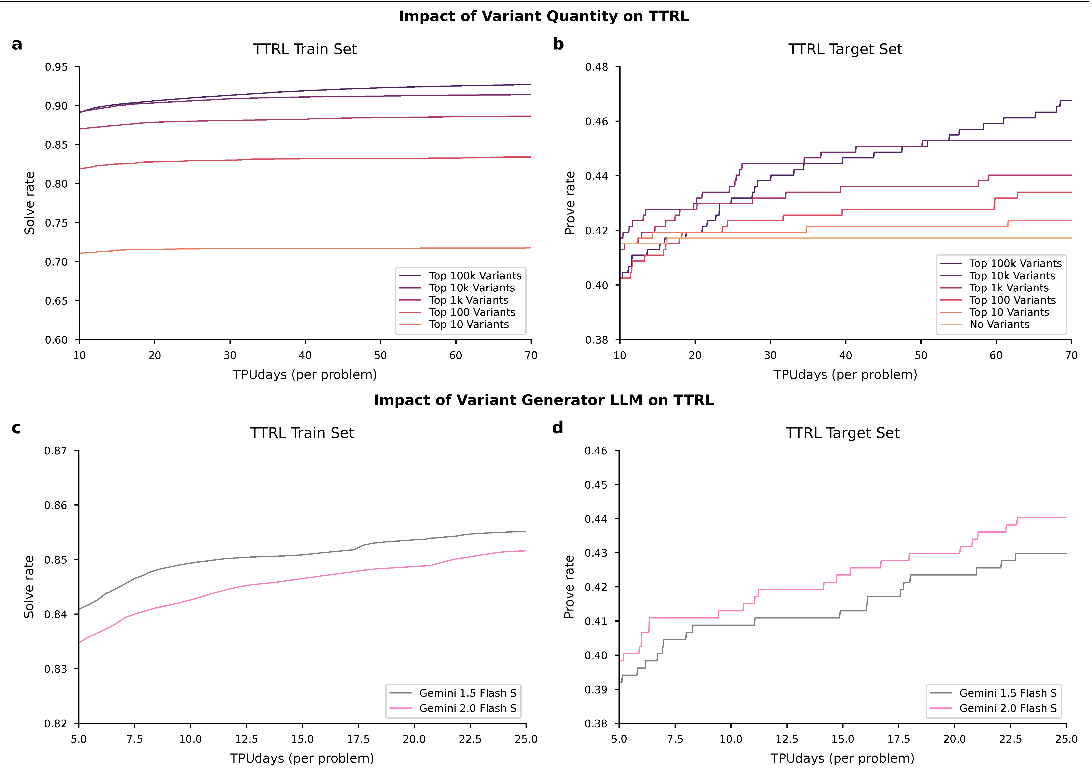
\includegraphics[width=\linewidth]{../papers/translations/alphaproof/assets/edfig3.pdf}\end{center}
\phantomsection
\noindent\textbf{扩展数据图 3. 改变合成变式数量及变式生成 LLM 的 TTRL 消融.}\paperlabel{扩展数据 3}{alphaproof-edfig3}
a, 增加课程变式数, 从 Top 10 到 Top 100k, 提高 TTRL 训练集内已解决变式比例. b, 更多合成变式持续提高目标题最终证明率, 展示更大问题专属变式集的显著益处. c, Gemini 1.5 Flash S (灰) 的训练变式解题率高于更强 Gemini 2.0 Flash S (粉), 提示后者变式可能构成更难课程. d, Gemini 2.0 Flash S 生成变式使目标题证明率显著更高, 说明该课程确实更有效.

\noindent\textbf{图中文字对应.} Impact of Variant Quantity on TTRL: 变式数量对 TTRL 的影响; Impact of Variant Generator LLM on TTRL: 变式生成 LLM 对 TTRL 的影响; TTRL Train Set: TTRL 训练集; TTRL Target Set: TTRL 目标集; Solve rate: 解题率; Prove rate: 证明率; TPUdays (per problem): 每题 TPU 日; Top 100k、Top 10k、Top 1k、Top 100、Top 10 Variants: 排名前 100,000、10,000、1,000、100、10 个变式; No Variants: 无变式. 模型名、曲线和全部坐标值保持原样.

\begin{center}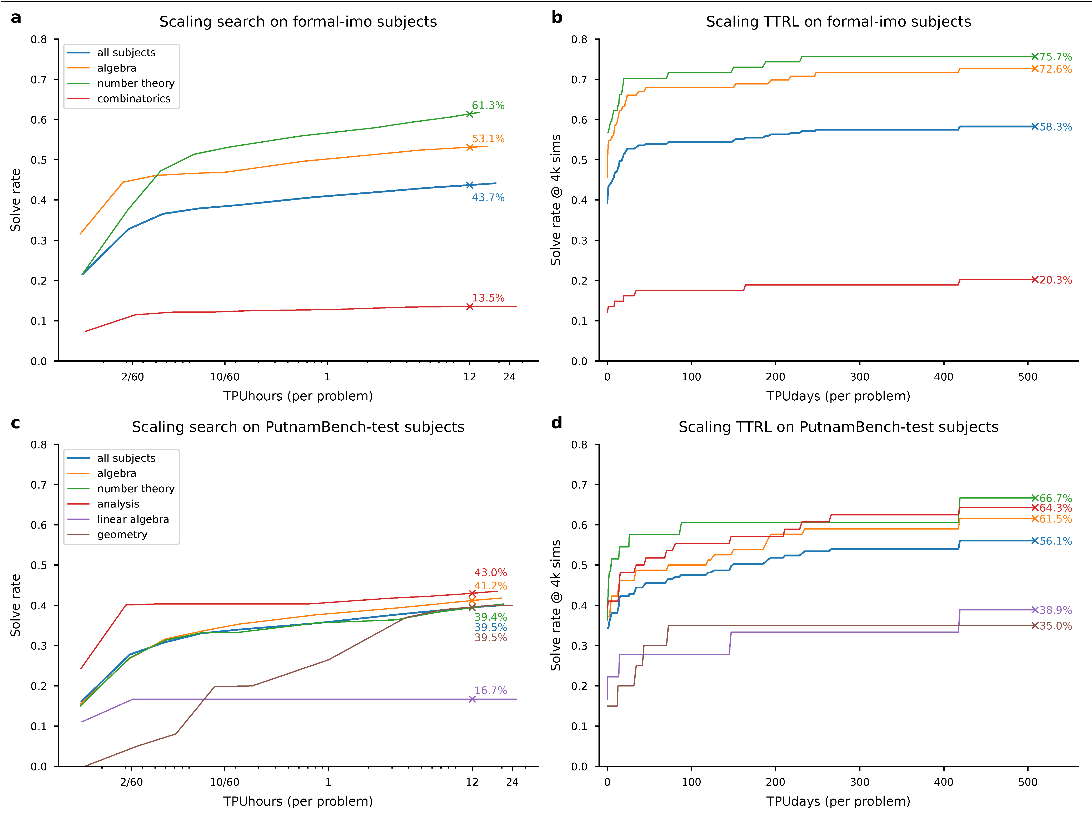
\includegraphics[width=\linewidth]{../papers/translations/alphaproof/assets/edfig4.pdf}\end{center}
\phantomsection
\noindent\textbf{扩展数据图 4. formal-imo 与 PutnamBench-test 按数学主题划分的推断扩展动态.}\paperlabel{扩展数据 4}{alphaproof-edfig4}
按主题细分两个基准的树搜索和 TTRL 解题率扩展. 粗蓝线为总体基准表现, 细线为具体主题表现.

\noindent\textbf{图中文字对应.} a、b 为 formal-imo 主题上的搜索、TTRL 扩展; c、d 为 PutnamBench-test 主题上的搜索、TTRL 扩展. All subjects: 全主题; algebra: 代数; number theory: 数论; combinatorics: 组合; analysis: 分析; linear algebra: 线性代数; geometry: 几何. Solve rate: 解题率; Solve rate @ 4k sims: 4,000 次模拟解题率; TPUhours (per problem)、TPUdays (per problem): 每题 TPU 小时、每题 TPU 日. 所有百分数、刻度及曲线原样保留.

\begin{center}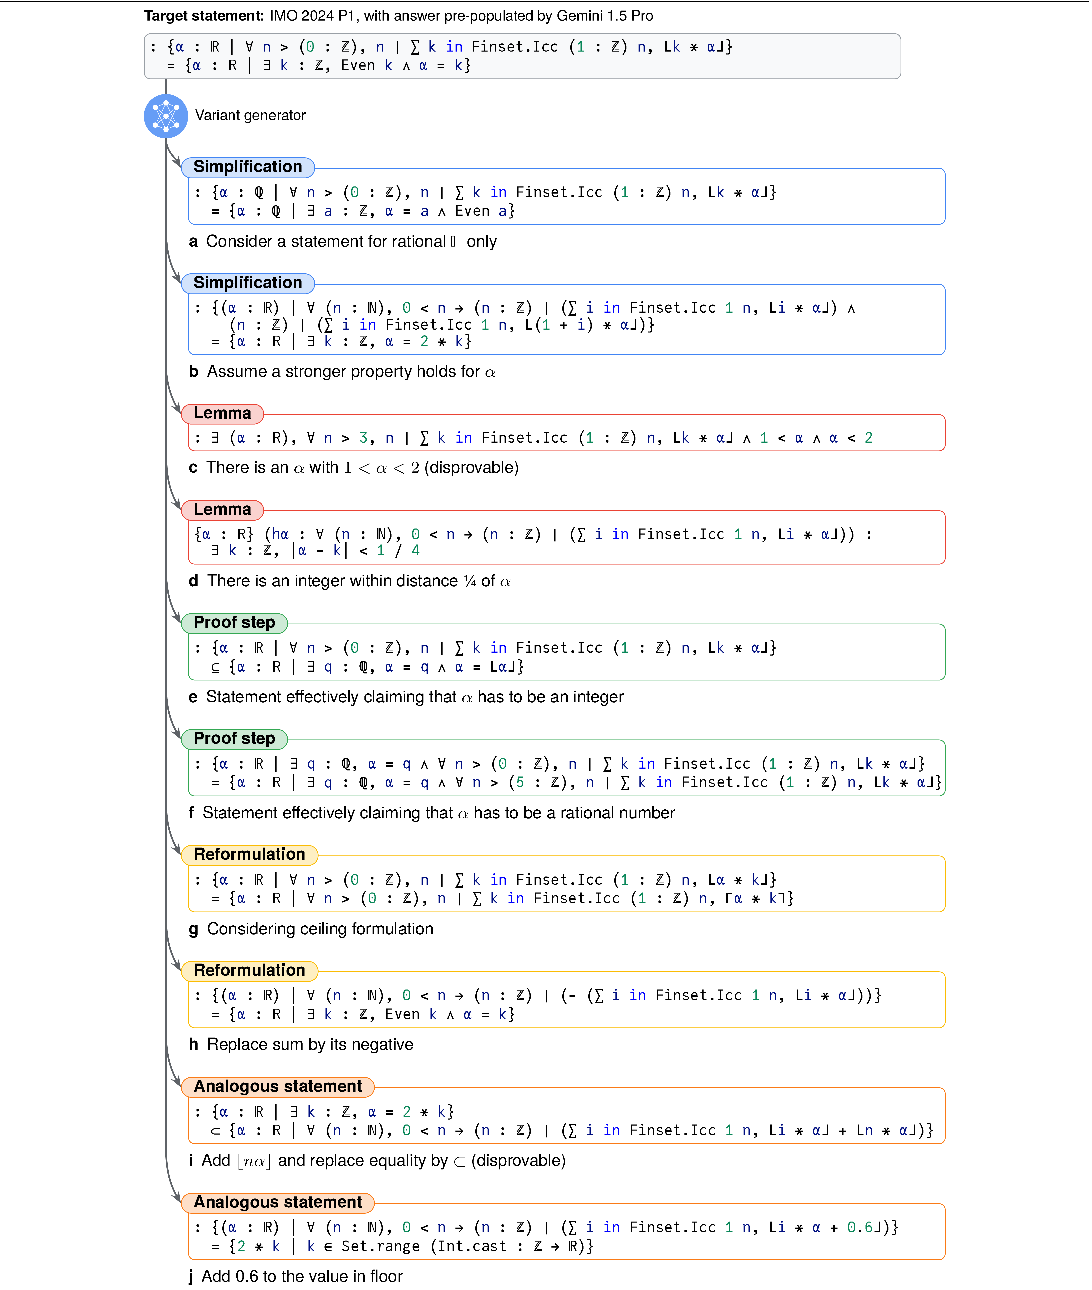
\includegraphics[width=\linewidth]{../papers/translations/alphaproof/assets/edfig5.pdf}\end{center}
\phantomsection
\noindent\textbf{扩展数据图 5. AlphaProof 为 IMO 2024 P1 自动生成的合成变式样例.}\paperlabel{扩展数据 5}{alphaproof-edfig5}
这些 Lean 变式在 TTRL 自动创建, 作者在此加标签和描述, 展示简化、提出引理、证明步骤、重新表述、探索类比等多样启发式. 处理这些变式帮助理解目标, 使证明智能体适应具体问题.

\noindent\textbf{图内文字完整中译.} Target statement: 目标命题, IMO 2024 P1, 答案由 Gemini 1.5 Pro 预先填入. Variant generator: 变式生成器. a, Simplification (简化): 只考虑有理数的命题. b, Simplification: 对 $\alpha$ 假设更强性质. c, Lemma (引理): 存在 $1<\alpha<2$ 的 $\alpha$, 此命题可反驳. d, Lemma: 在距 $\alpha$ 小于 $1/4$ 的范围有整数. e, Proof step (证明步骤): 实质声称 $\alpha$ 必须为整数的命题. f, Proof step: 实质声称 $\alpha$ 必须为有理数的命题. g, Reformulation (重新表述): 考虑上取整形式. h, Reformulation: 用和式的相反数替换和式. i, Analogous statement (类比命题): 加入 $\lceil n\alpha\rceil$ 并用整除替换, 该命题可反驳. j, Analogous statement: 对下取整中的值加 0.6. 目标和 a--j 每个变式的完整 Lean 代码、量词、数值、集合、有限求和、上下取整符号及颜色, 全部保持原图, 不将可反驳变式改成正确命题.

\begin{center}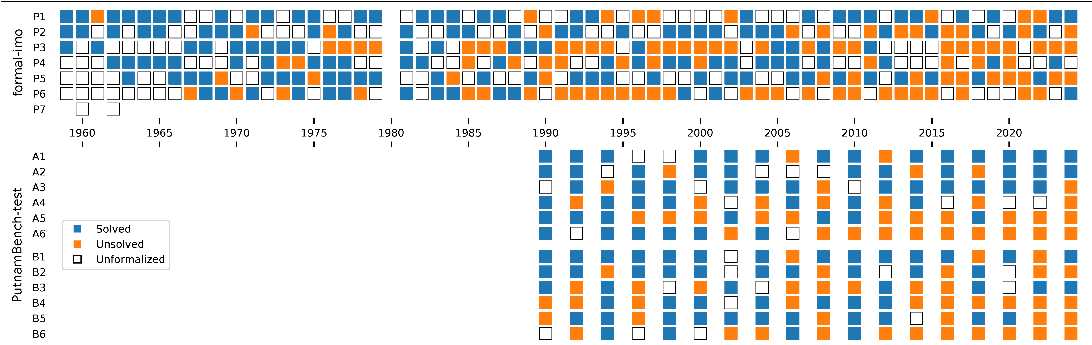
\includegraphics[width=\linewidth]{../papers/translations/alphaproof/assets/edfig6.pdf}\end{center}
\phantomsection
\noindent\textbf{扩展数据图 6. formal-imo 与 PutnamBench-test 在 TTRL 结束或主 RL 时解决的问题.}\paperlabel{扩展数据 6}{alphaproof-edfig6}
蓝为已解决, 橙为未解决, 白为未形式化. IMO 因政治原因在 1980 年未举行.

\noindent\textbf{图中文字对应.} Solved: 已解决; Unsolved: 未解决; Unformalized: 未形式化. 每个年份、题号 P1--P7、A1--A6、B1--B6 及对应颜色方格保持原样; 未形式化不同于尝试后未解.

\clearpage
\noindent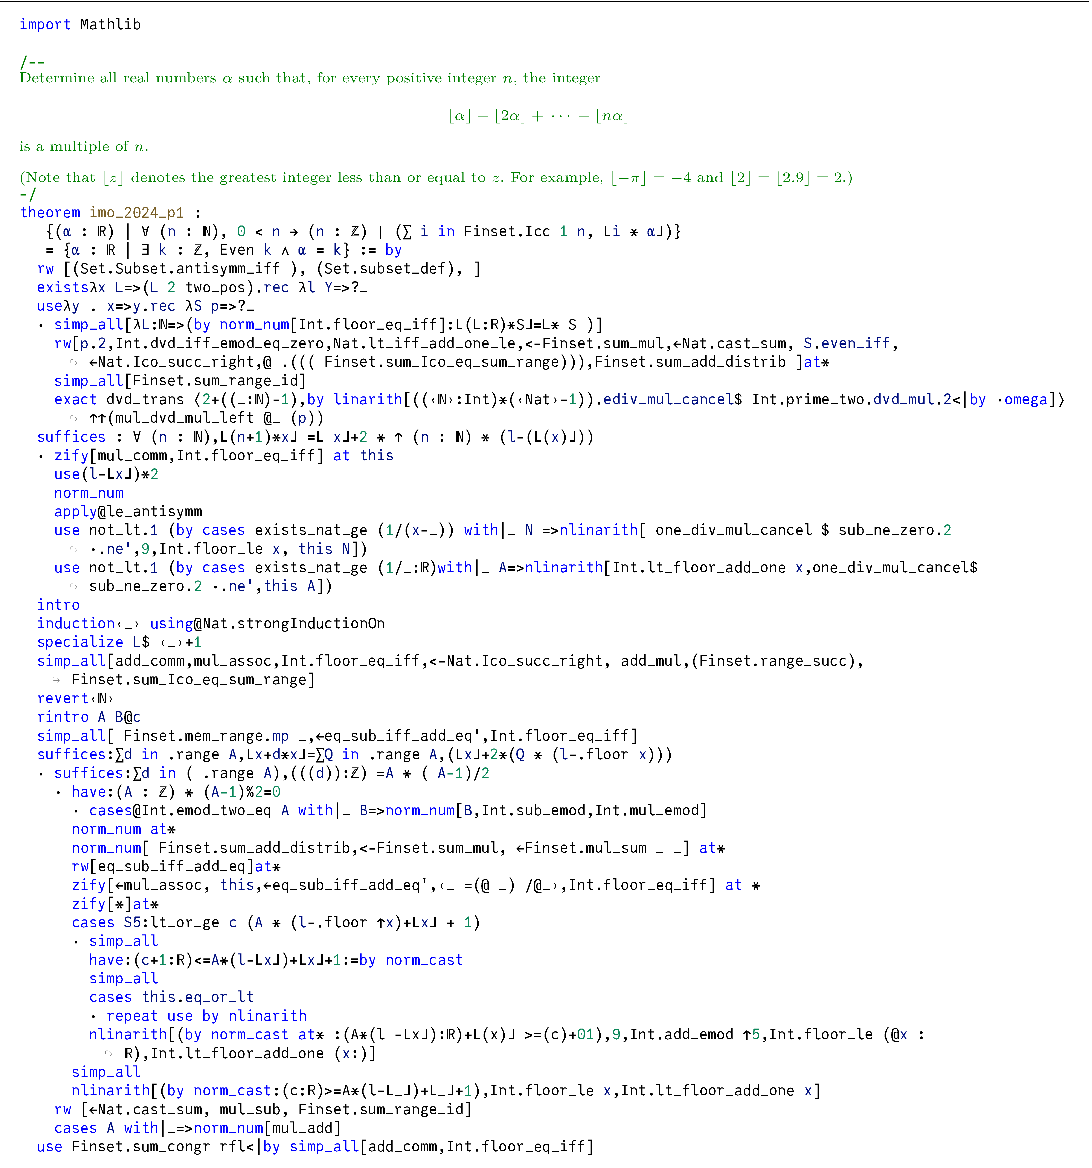
\includegraphics[width=\linewidth]{../papers/translations/alphaproof/assets/edfig7.pdf}\par
\phantomsection
\noindent\textbf{扩展数据图 7. AlphaProof 找到的 IMO 2024 P1 完整证明.}\paperlabel{扩展数据 7}{alphaproof-edfig7}
按第 6.4 节协议找到. 本图及扩展数据图 8、9 的交互版本见文献\cite{alphaproof-ref28}, 可查看全部中间 Lean 目标状态. 609 名学生中 413 人完整解出了此代数题\cite{alphaproof-ref27}. 图改编自文献\cite{alphaproof-ref28}.

\noindent\textbf{代码题面注释完整中译.} 求所有实数 $\alpha$, 使每个正整数 $n$ 都满足整数
\[
\lfloor\alpha\rfloor+\lfloor2\alpha\rfloor+\cdots+\lfloor n\alpha\rfloor
\]
是 $n$ 的倍数. $\lfloor z\rfloor$ 表示不大于 $z$ 的最大整数, 例如 $\lfloor-\pi\rfloor=-4$, $\lfloor2\rfloor=\lfloor2.9\rfloor=2$. 原图从 \texttt{import Mathlib} 到最后一个 tactic 的完整代码、全部量词、证明分支和形式解集均保留; 形式命题的解集表述为偶整数. 此处仅翻译注释, 不把代码改为另一份证明, 也不声称本译文重新编译验证过它.

\clearpage
\noindent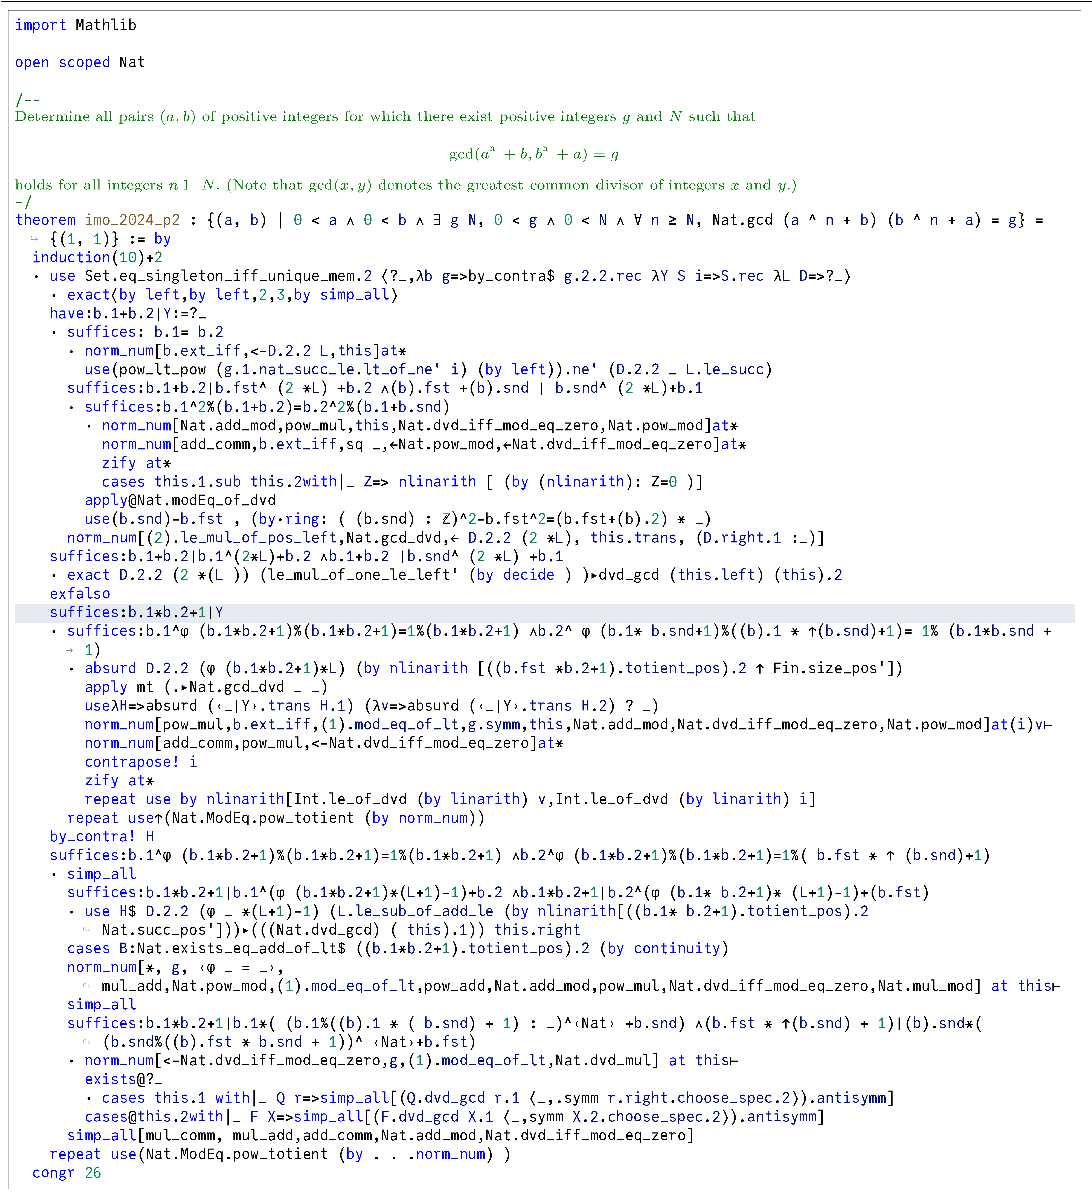
\includegraphics[width=\linewidth]{../papers/translations/alphaproof/assets/edfig8.pdf}\par
\phantomsection
\noindent\textbf{扩展数据图 8. AlphaProof 找到的 IMO 2024 P2 完整证明.}\paperlabel{扩展数据 8}{alphaproof-edfig8}
按第 6.4 节协议找到. 证明关键是考虑 $ab+1$ 的性质, 例如它整除 $g$, 在高亮行可见. 609 名学生中 156 人完整解出了此数论题\cite{alphaproof-ref27}. 图改编自文献\cite{alphaproof-ref28}.

\noindent\textbf{代码题面注释完整中译.} 求全部正整数对 $(a,b)$, 使存在正整数 $g,N$, 对所有整数 $n\ge N$ 均有
\[
\gcd(a^n+b,b^n+a)=g.
\]
$\gcd(x,y)$ 表示整数 $x,y$ 的最大公因数. 原图完整保留 \texttt{import Mathlib}、\texttt{open scoped Nat}、解集 $\{(1,1)\}$ 的形式定理、全部代码与高亮行.

\begin{remark}
译注: 原 PDF 英文题面注释中 $n$ 与 $N$ 之间的比较符号显示不完整. 紧接的 Lean 正式命题明确为 $\forall n\ge N$; 上文据该代码转录为 $n\ge N$. 原图仍按原件保留, 没有修补图像或声称图内字形已恢复.
\end{remark}

\clearpage
\noindent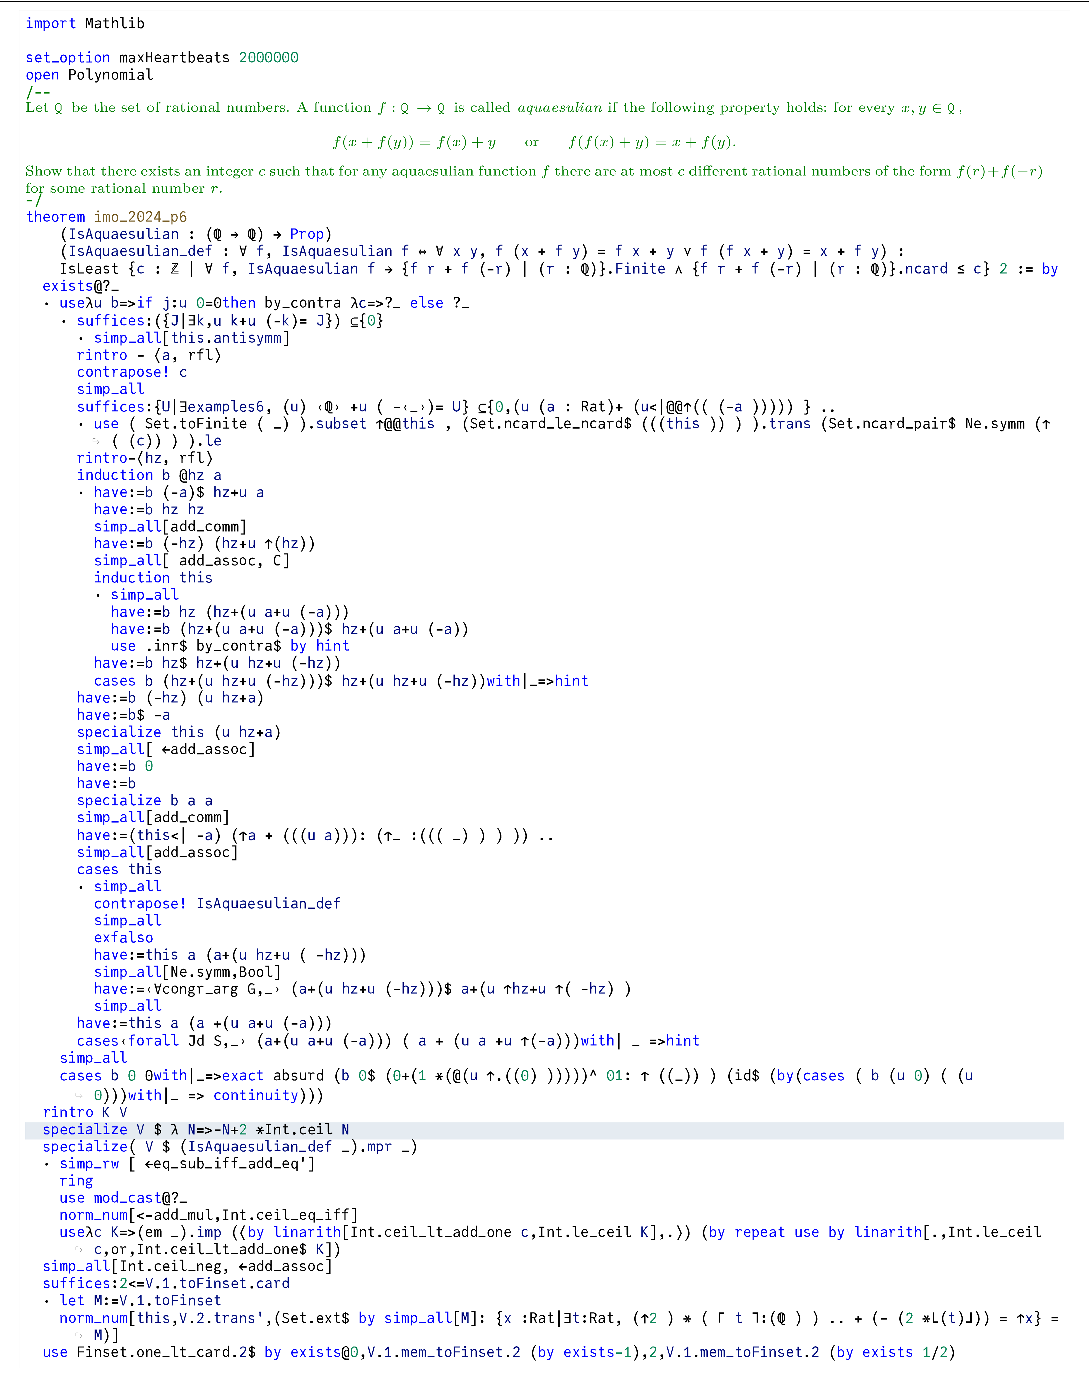
\includegraphics[width=\linewidth]{../papers/translations/alphaproof/assets/edfig9.pdf}\par
\Needspace{3\baselineskip}
\phantomsection
\noindent\textbf{扩展数据图 9. AlphaProof 找到的 IMO 2024 P6 完整证明.}\paperlabel{扩展数据 9}{alphaproof-edfig9}
按第 6.4 节协议找到. 高亮行展示关键见解: 构造 $f(x)=-x+2\lceil x\rceil$. 609 名学生中只有 5 人完整解出了此代数题\cite{alphaproof-ref27}. 图改编自文献\cite{alphaproof-ref28}.

\noindent\textbf{代码题面注释完整中译.} 设 $\mathbb Q$ 为有理数集. 函数 $f:\mathbb Q\to\mathbb Q$ 若对每个 $x,y\in\mathbb Q$ 满足下列性质, 称为 aquaesulian:
\[
f(x+f(y))=f(x)+y\quad\text{或}\quad f(f(x)+y)=x+f(y).
\]
证明存在整数 $c$, 使对任一 aquaesulian 函数 $f$, 当有理数 $r$ 变化时, $f(r)+f(-r)$ 至多有 $c$ 个不同的有理值. 原图 \texttt{set\_option maxHeartbeats 2000000}、\texttt{open Polynomial}、\texttt{IsAquaesulian}、\texttt{IsAquaesulian\_def}、\texttt{IsLeast} 命题及最小值 2 的完整形式代码全部保留. 构造反例函数的高亮行与后续证明没有省去, 未重新执行.

\Needspace{6\baselineskip}
\phantomsection
\noindent\textbf{扩展数据表 1. 自动形式化在各含五十道代表性 IMO、Putnam 题的内部基准上的表现.}\paperlabel{扩展数据 1}{alphaproof-edtable1}
\begin{center}
\begin{tabular}{lrrrrrr}
\toprule
 & 代数 & 数论 & 组合 & 几何 & 全主题 & pass@k ($k$ 次研究)\\
\midrule
IMO & $81.3\%$ & $76.9\%$ & $33.3\%$ & 不包含 & $60.0\%$ & $96\%$ ($k=29$)\\
Putnam & $61.9\%$ & $72.7\%$ & $60.0\%$ & $54.6\%$ & $64.0\%$ & $98\%$ ($k=16$)\\
\bottomrule
\end{tabular}
\end{center}
\noindent\textbf{原表注.} 这些基准的具体题目见补充表 5. 除最后一列外全部数字是 pass@1; 最后一列为在我们任一次共 $k$ 次研究中正确形式化的问题比例, 由 Lean 专家评判.

\Needspace{6\baselineskip}
\phantomsection
\noindent\textbf{扩展数据表 2. AlphaProof 各配置在全部基准上的详细表现.}\paperlabel{扩展数据 2}{alphaproof-edtable2}
\begin{center}
\begin{tabular}{p{2.7cm}p{1.9cm}rrrrr}
\toprule
配置 & 每题预算 & miniF2F-valid & miniF2F-test & formal-imo & Putnam 训练 & Putnam 测试\\
\midrule
AlphaProof & 2 TPU 分钟 & $96.0\%$ & $96.3\%$ & $33.2\%$ & $35.4\%$ & $27.9\%$\\
AlphaProof & 12 TPU 小时 & $97.1\%$ & $97.7\%$ & $43.7\%$ & $48.7\%$ & $39.5\%$\\
AlphaProof 加 TTRL & 50 TPU 日 & $99.6\%$ & $97.5\%$ & $53.9\%$ & -- & $45.5\%$\\
AlphaProof 加 TTRL & 500 TPU 日 & $100.0\%$ & $99.6\%$ & $58.3\%$ & -- & $56.1\%$\\
\bottomrule
\end{tabular}
\end{center}
\noindent\textbf{原表注.} “每题计算预算”为原文图 4a 定义的平均计算成本. miniF2F\cite{alphaproof-ref20} 的 valid 划分全部 $100\%$ 已证明. PutnamBench-train 与 PutnamBench-test\cite{alphaproof-ref21} 的树搜索具有相似扩展性质. TTRL 没有用于 PutnamBench-train. 表中 Putnam 训练、测试分别是原文的 PutnamBench-train、PutnamBench-test.

\begin{remark}
译注: 原文主表 1 的 12 TPU 小时 PutnamBench-test 为 $39.4\%$, 本扩展表及原文图 4 为 $39.5\%$. 本译文保留各自原值, 不统一改写. 原文图 4 与扩展表在 miniF2F-valid 的某些标注也不完全相同, 均按各原件保留.
\end{remark}

